\begin{document}
%=================================================================
%                           Start Document
%=================================================================
\section{Implementation}
\lhead{Implementation} % section header
\setstretch{1.6}
\lhead{Implementation - Software Refactoring}
\subsection{Software Refactoring}
As mentioned introduction wise this project builds upon the work and code base originally developed for FES with the LegoPress \cite{olivier_legopress_2014} and further developed by a previous student. However the code quality was poor with thousands of lines of code and multiple functionalities all implemented in one file and one class. Therefore before continuing on with the project a proper refactoring of the code was necessary. The goal being to save time in the long run by creating modular, robust, readable code that could later be further built upon for use in clinical trials.

The software is written in C++ in QT.

\subsubsection{Documentation}

In order to understand the code it was decided that the first step would be to create documentation, specifically graphical representations of the interactions and hierarchy. To accomplish the code was documented and edited so that it would be compatible with doxygen. Doxygen is a documentation generation tool that automatically creates software documentation from annotated source code in HTML.

\begin{figure} [H]
    \centering
    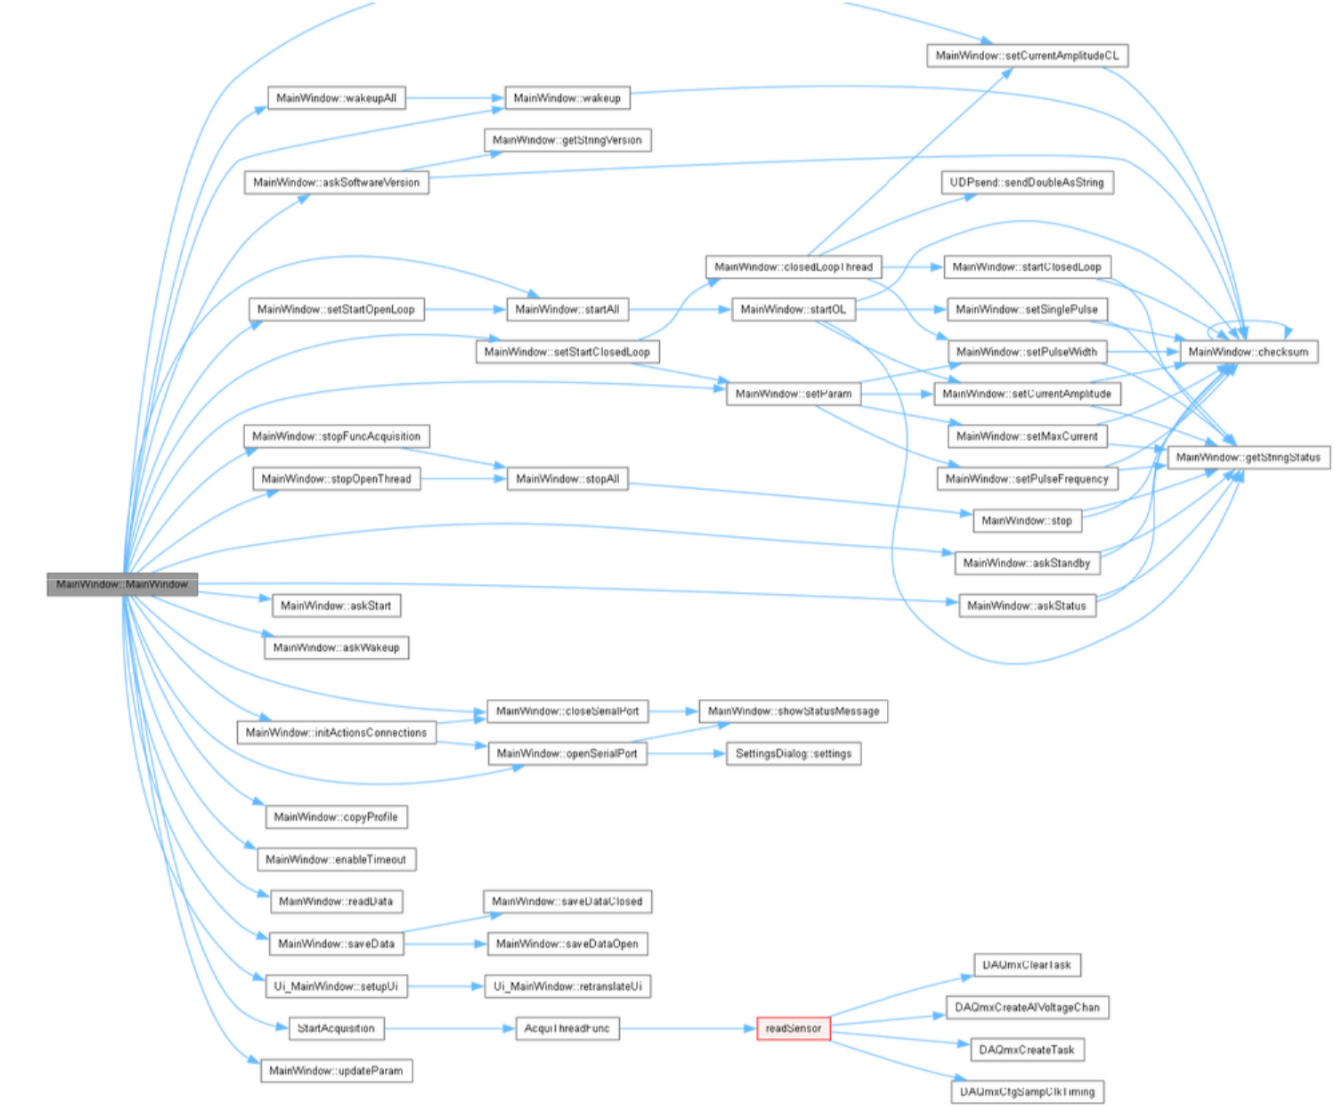
\includegraphics[width=0.9\linewidth]{images/oldDoxy.png}
    \caption{Original callgraph for mainwindow function before refactoring, generated by doxygen}
    \label{fig:oldDoxy}
\end{figure}

After the code had been documented and visualized in doxygen it became possible to see the call graphs and interactions such as in figure \ref{fig:oldDoxy}. This sped up the process of understanding the code thus laying important groundwork for the clearning and modularization step.

\subsubsection{Modularization}
In order to improve the code quality, a modularization and cleaning of the code base was necessary. The code was refactored and divided into classes based mainly on the code quality principles laid out in Code Complete by Steve McConnel \cite{steve_mcconnell_code_nodate}. This includes having clearly defined, minimal interfaces. This is accomplished by using the signal slot mechanism inbuilt into QT, which allows for communication between objects in an event-driven, decoupled manner. Another core concept is organizing modules hierarchically, where higher-level modules depend on lower-level modules but not the reverse. 

\begin{figure} [h]
    \centering
    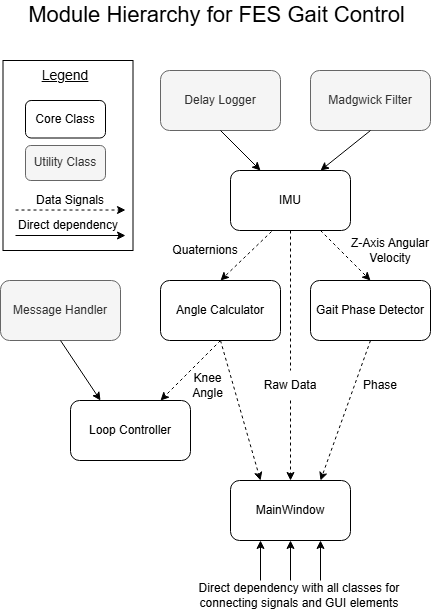
\includegraphics[width=0.6\linewidth]{images/gaitcontrol.png}
    \caption{Module hierarchy after refactoring}
    \label{fig:modulehier}
\end{figure}

A visualization of the hierarchy after refactoring can be seen in figure \ref{fig:modulehier} and description of each class are in table \ref{tab:class-overview}. Previously, all loop controller and IMU functionality and serial communication and bit handling was all done in the mainwindow class. There was also code only relevant for the legopress still in the mainwindow class. That code for the legopress was removed and the usable, existing code was moved to their appropriate classes which were the message handler, LoopController and MainWindow. All old IMU functionality was also removed since part of the project involved changing out the old wired IMUs with the new wireless IMUs developed in the lab. The final architecture has a high cohesion and low coupling resulting in readable, scalable, testable and reusable code.


\lhead{Implementation - Functional Electrical Stimulation Setup}
\subsection{Functional Electrical Stimulation Setup}

\subsubsection{Hardware}
The hardware used for the functional electrical stimulation was the StimWave developed at the REHassist lab. It consists of 10 channels where each channel is controlled via an RS-232 line in a master/slave manner. Each electrostimulation channel (slave) has its own adress and every command from the FES Gait Control software (master), is dedacted to only one channel. Meaning that each channel can be used in order to apply FES to a muscle. There is a protocol that describes what each 3 byte command encodes. Using this encoding the pulse frequency, pulse width and current amplitude may be adjusted. Along with other commands such as start, stop and status commands. 

\begin{figure} [h]
    \centering
    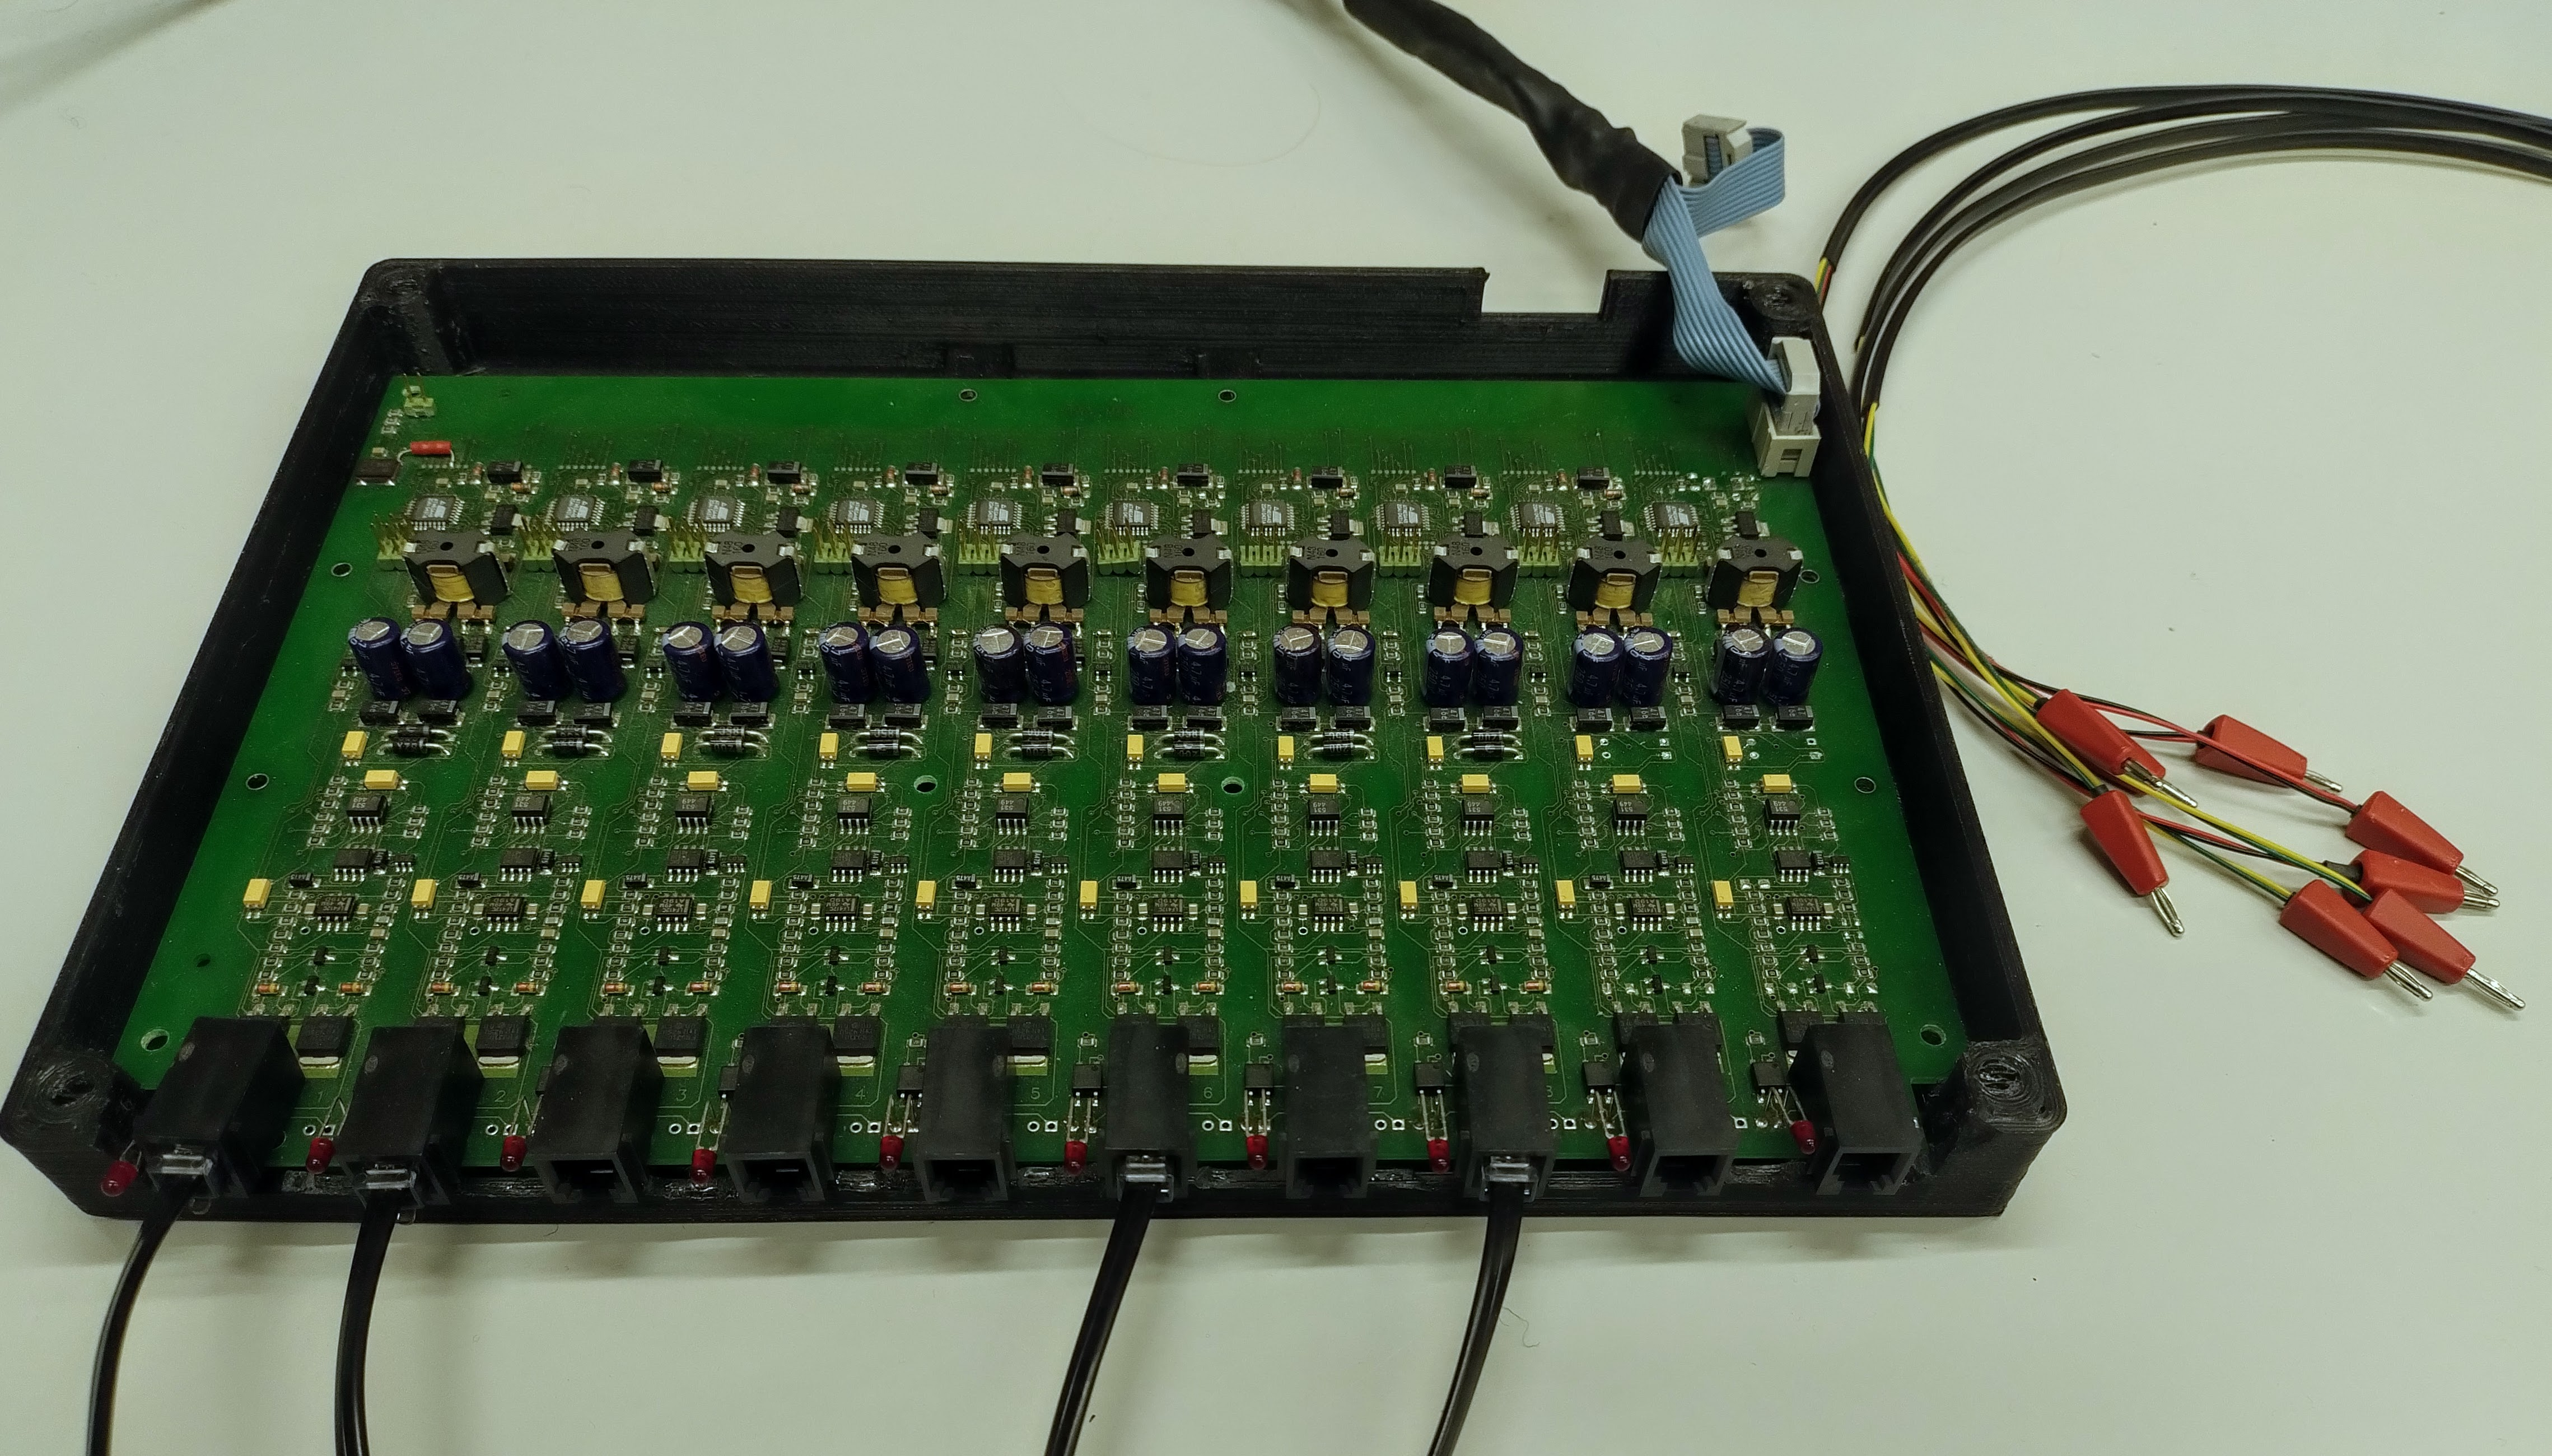
\includegraphics[width=0.8\linewidth]{images/stimwave.jpg}
    \caption{StimWave hardware used}
    \label{fig:enter-label}
\end{figure}

However the selection code for the pulse width and frequency had been changed since the implementation used in the original code base. The first step before using this hardware for FES was therefore to adjust the translation of pulsewidth and frequency to the correct 7 bit selection code thereby creating the correct 3 byte commands in the \texttt{MessageHandler} class. These changes were verified by using an oscilloscope before moving on to FES. 


\subsubsection{Stimulation waveform}
Stimulus waveforms are generally monophasic or biphasic. Monophasic waveforms consist of a single phase of electrical current delivered in one polarity, while Biphasic waveforms consist of a cathodic phase followed by an anodic phase. This mitigates the buildup of charge at the electrode-tissue interface by ensuring that the net charge delivered over time is zero, effectively reducing the risk of tissue damage as compared to monophasic waveforms \cite{peckham_functional_2005}. The biphasic rectangular stimulation is the most commonly used, as it offers the best force-amplitude ratio
\cite{lynch_functional_2008}. For these reasons the balanced biphasic rectangular waveform was chosen for the stimulation protocol.
 \begin{figure} [H]
     \centering
     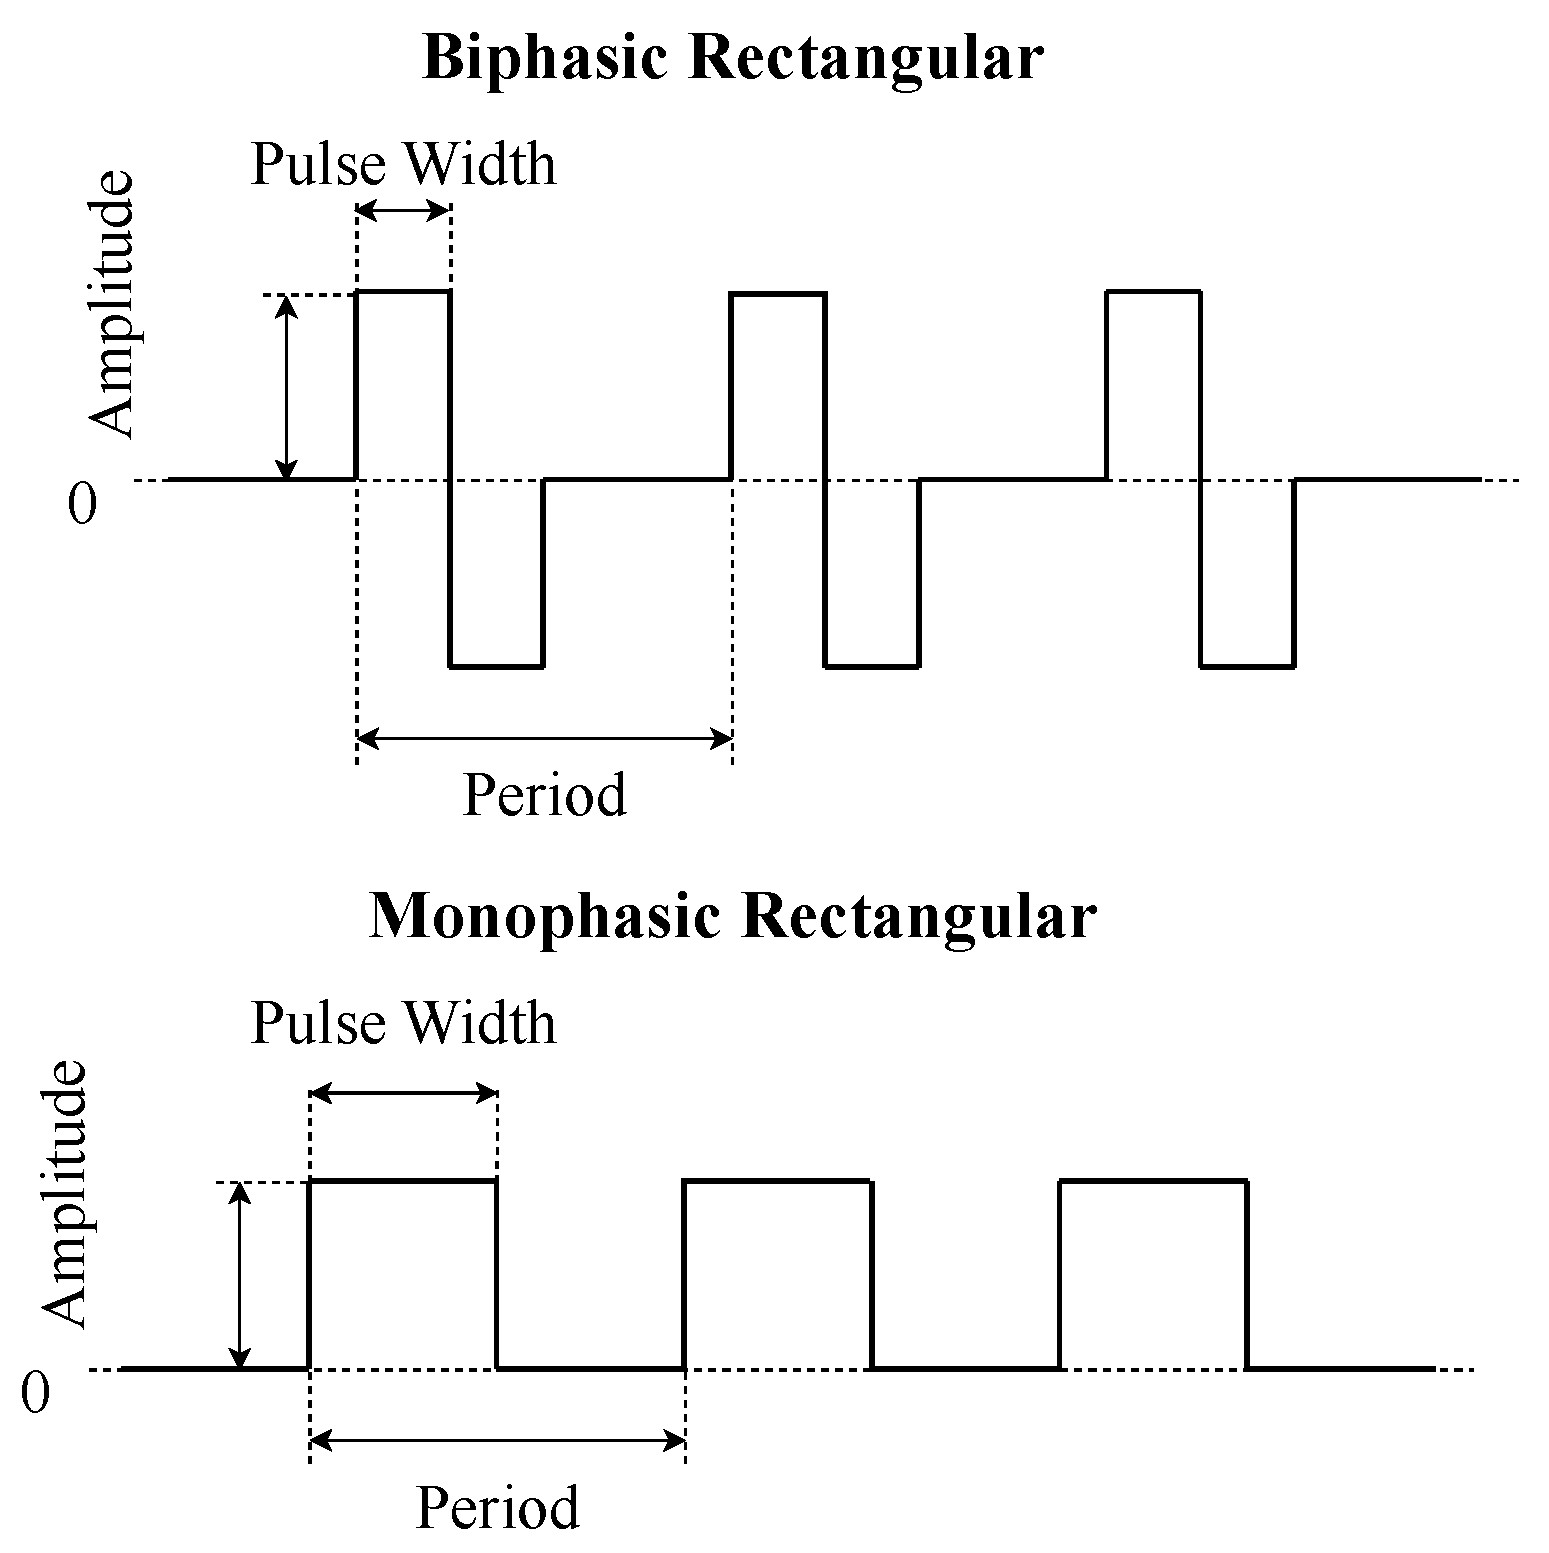
\includegraphics[width=0.6\linewidth]{images/twowaveform.jpg}
     \caption{Caption}
     \label{fig:enter-label}
 \end{figure}
 

\subsubsection{Stimulation frequency}
The stimulation frequency affects the strength of the contraction and its quality. A higher frequency will lead to the force produced by each subsequent pulse being added so that the mean force of the contraction is greater than that produced by a single twitch. Further increase in frequency results in sustained contraction which produces a smooth movement instead of individual twitches. The minimum frequency required to induce fairly consistent contraction is between 16 and 20 Hz \cite{marquez-chin_functional_2020}. A smoother contraction is also more comfortable for the patient. However one should not use a higher frequency than necessary since it has been observed that fatigue accumulated in a muscle is related to the number of pulses received \cite{bigland-ritchie_muscle_2000}. 

\begin{figure} [H]
    \centering
    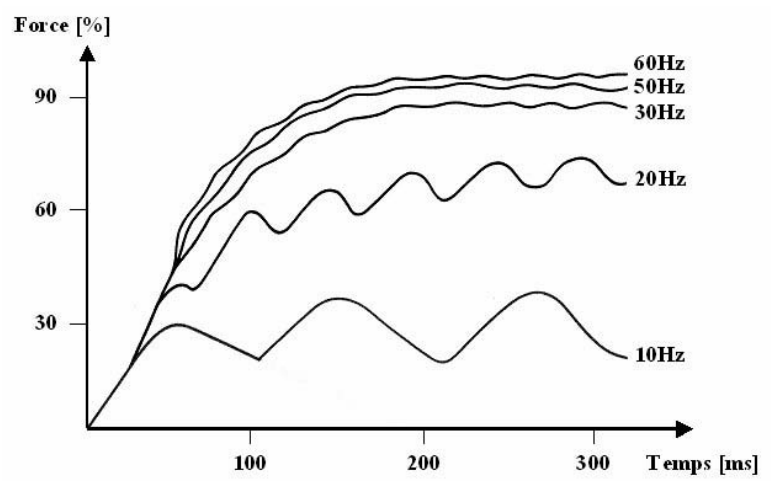
\includegraphics[width=0.7\linewidth]{images/stimfreq.png}
    \caption{Effect of stimulation frequency on force generation \cite{metrailler_systeme_2005}}
    \label{fig:stimfreq}
\end{figure}

When choosing the stimulation frequency the aim was therefore to choose the lowest frequency that still produced sustained contractions. In a clinical environment, the typical range of frequencies is around 20-50Hz, and during literature review it was observed that the majority of teams using FES on gait are using a stimulation frequency around 40Hz \cite{aout_effects_2023}. Therefore the same 40Hz stimulation frequency was chosen for this project.



\subsubsection{Stimulation intensity }
The stimulation intensity is determined by the pusle duration as well as the pulse amplitude. To vary the intesity one is therefore often kept constant while the other is tuned. 

 \todo{explain better why modulating w amplitude?} 
The pulse duration (pulse width) is the timespan of the stimulation pulse. Higher pulse widths result in more pronounced contraction and enable deeper tissue penetration of the stimulation . Most sudies attempting FES for gait employ pulse widths spanning from 200 to 400 \micro s. The majority keep the pulse duration fixed at 300 \micro s and only vary the amplitude in order to set the stimulation intensity.\cite{aout_effects_2023}

The amplitude of the stimulation determines which muscles are contracted and the strength of the contraction \cite{marquez-chin_functional_2020}. Larger amplitudes a larger proportion of the muscle fibers, including those located deeper. 

There are several clinically important values for the amplitude that can be identified. The first is the motor threshold, which is the minimum intensity  that results in a visible muscle contraction, even if it does not produce a movement \cite{marquez-chin_functional_2020}. The second is the Maximum tolerable intensity, which is the maximum amplitude that the person can sustain without pain. Finally there is the operational stimulation amplitude, which is the amplitude that produces the intended functional movement needed for the gait cycle. 

These thresholds are highly variable and dependent on both muscle and subject, therefore they are determined here experimentally by slowly ramping up the amplitude for one muscle at a time. Noting when a motor threshold is reached, when the maximum tolerable intensity is reached and based on these values and feedback from the patient a operational stimulation amplitude is set somewhere between the thresholds. This is expanded upon in the sections relating to the open loop and closed loop implementations.

\subsubsection{Electrode configuration}
There are two main configuration for electrical activation of neuromuscular tissue. There is bipolar stimulation in which each stimulation cite has an active electrode placed near the peripheral nerve and a reference electrode close by. The other configuration is monopolar where the return electrode is placed in a remote area near less excitable tissue \cite{peckham_functional_2005}. 
This approach reduces the number of leads and electrodes required, however for multichannel systems bipolar stimulation may allow greater selectivity of activation because each electrode par creates a more localized electric field \cite{grandjean_recruitment_1986}. For this reason and also since there were already cables compatible with this configuration available bipolar stimulation was chosen.



















%=================================================================
%                           End Document
%=================================================================
\end{document}